

%\usepackage{fancyhdr}
%\pagestyle{fancy}
%\rhead{\includegraphics[width = 1\textwidth]{marca.jpg}}


\usepackage{geometry}
\geometry{a4paper, left=10mm, right=10mm, bottom=15mm, top=16mm}
\usepackage{setspace}
\doublespacing
\usepackage[spanish]{babel}
\usepackage{color}
\usepackage{xcolor}
\usepackage{framed}
\colorlet{shadecolor}{gray!20}
\setcounter{secnumdepth}{0}
\usepackage{sectsty}


\chapternumberfont{\Large}
\chaptertitlefont{\Large}
\setcounter{tocdepth}{5}
\setcounter{secnumdepth}{5}
\setlength{\footskip}{20pt}%Esto sube el número de página
\usepackage{graphics}
\usepackage{setspace} %paquete para el doble espaciado
%\doublespacing %inicia el doble espaciado
 %Esto quita el punto final en la numeracion de cada seccion
\usepackage{tocloft}

\usepackage{titlesec}
\titleformat{\section}
{\Large\bfseries}{\thesection}{0.5em}{}
\titleformat{\subsection}
{\large\bfseries}{\thesubsection}{0.5em}{}
\titleformat{\subsubsection}
{\normalsize\bfseries}{\thesubsubsection}{0.5em}{}
\titleformat{\paragraph}
{\normalsize\bfseries}{\theparagraph}{0.5em}{}
\renewcommand\cftsecaftersnum{}
\renewcommand\thesection{\arabic{section}}
\renewcommand\thesubsection{\thesection.\arabic{subsection}}
\usepackage{caption}
\usepackage{fancyhdr}
\pagestyle{fancy}
\fancyhf{}
\fancyhead[R]{\rightmark}
\fancyfoot[R]{\thepage}
\fancyfoot[C]{Teléfono  8731-4699    |   info@cesargamboasanabria.com  |   www.cesargamboasanabria.com}
\setlength{\headheight}{21.9pt}
\renewcommand\sectionmark[1]{%
\markright{\thesection\ #1}}
\renewcommand{\footrulewidth}{0.4pt}
\renewcommand{\headrulewidth}{0pt}

%\renewcommand{\footnoterule}{%
%  \kern -1pt
%  \hrule width \textwidth height 1pt
%  \kern 4pt
%}


%MARCA DE AGUA
\usepackage{graphicx}
 \usepackage{fancyhdr}
  \pagestyle{fancy}
  \setlength\headheight{28pt}
   \fancyhead[L]{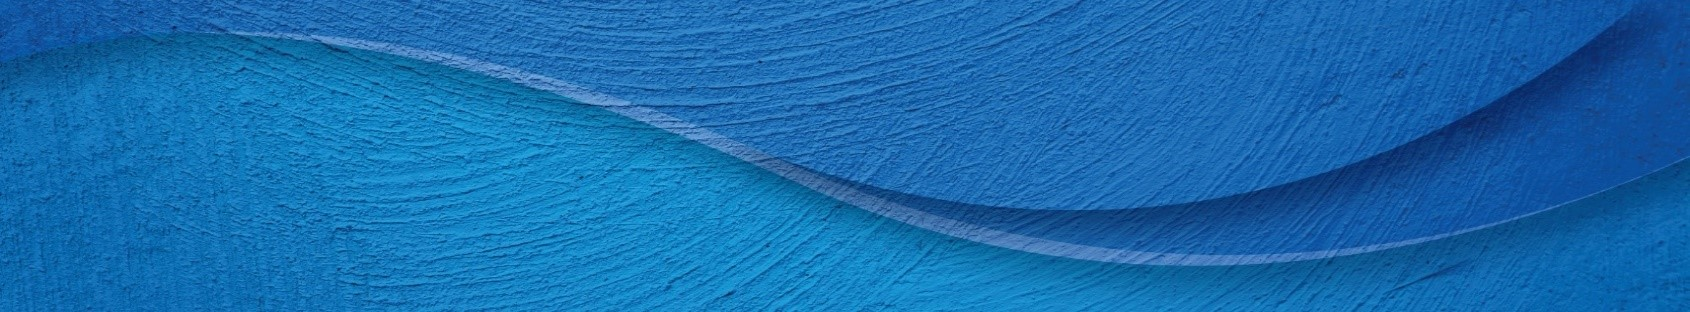
\includegraphics[width=19cm]{cabecera.jpg}}
   \fancyfoot[LE,RO]{}

\usepackage{booktabs}
\usepackage{longtable}
\usepackage{array}
\usepackage{multirow}
\usepackage{wrapfig}
%\usepackage{float}
\usepackage{colortbl}
\usepackage{pdflscape}
\usepackage{tabu}
\usepackage{threeparttable}
\usepackage{threeparttablex}
\usepackage[normalem]{ulem}
\usepackage{makecell}
\usepackage{xcolor}

\usepackage{tocloft}
\renewcommand{\cftsecleader}{\cftdotfill{\cftdotsep}}

%\renewcommand{\familydefault}{\sfdefault} %Para cambiar la fuente


%Para referenciar chunks
\usepackage{caption}
\usepackage{floatrow}
\floatsetup[figure]{capposition=top}
\floatsetup[table]{capposition=top}
\floatplacement{figure}{H}
\floatplacement{table}{H}
\captionsetup[table]{name=, labelformat=empty}

\DeclareNewFloatType{chunk}{placement=H, fileext=chk, name=}
\captionsetup{options=chunk}
\renewcommand{\thechunk}{Código~\arabic{chunk}}
\makeatletter
\@addtoreset{chunk}{section}
\makeatother


\usepackage{tikz}
\usetikzlibrary{calc}

\newcommand{\positiontextbox}[4][]{%
  \begin{tikzpicture}[remember picture,overlay]
%    \draw[step=0.5,gray!80!white] (current page.north west) grid (current page.south east); % For controlling
    \node[inner sep=10pt,right,#1] at ($(current page.north west) + (#2,-#3)$) {#4};
  \end{tikzpicture}%
}
